% questions.tex —— 2017 年·全国Ⅰ卷·文科 · 题目内容片段（无答案）
% 由 tools/generate_projects.py 依来源总账自 2017/2017_数学真题_文_试题.md 生成，勿手改（改源 MD 后重跑）


\begin{gknotice}
\textbf{ 卷种提示}：本卷为文理分科时代的旧结构，含\textbf{现已取消}的选做题（第 22/23 题）与\textbf{已删除}的程序框图考点（第 10 题）。适合\textbf{按知识点抽题}，不适合整套限时模拟。

\textbf{与同年理科卷重合}：第 4、10 题与第 18(1)、22、23 题与理科卷相同；第 19 题使用同一组数据但问法不同。
\end{gknotice}

\par\medskip

\gkpart{一、选择题}

\begin{gktip}
本题共 12 小题，每小题 5 分，共 60 分。
\end{gktip}

\begin{question}
\gkti{1}已知集合 $A=\{x\mid x<2\}$，$B=\{x\mid3-2x>0\}$，则\mbox{（　　）}

\begin{gkopts}(1)
\task A．$A\cap B=\left\{x\ \middle|\ x<\dfrac32\right\}$
\task B．$A\cap B=\varnothing$
\task C．$A\cup B=\left\{x\ \middle|\ x<\dfrac32\right\}$
\task D．$A\cup B=\mathbf R$
\end{gkopts}

\end{question}
\begin{question}
\gkti{2}为评估一种农作物的种植效果，选了 $n$ 块地作试验田。这 $n$ 块地的亩产量（单位：$\mathrm{kg}$）分别是 $x_1$，$x_2$，$\cdots$，$x_n$，下面给出的指标中可以用来评估这种农作物亩产量\textbf{稳定程度}的是\mbox{（　　）}

\begin{gkopts}(2)
\task A．$x_1,x_2,\cdots,x_n$ 的平均数
\task B．$x_1,x_2,\cdots,x_n$ 的标准差
\task C．$x_1,x_2,\cdots,x_n$ 的最大值
\task D．$x_1,x_2,\cdots,x_n$ 的中位数
\end{gkopts}

\end{question}
\begin{question}
\gkti{3}下列各式的运算结果为纯虚数的是\mbox{（　　）}

\begin{gkopts}(2)
\task A．$\mathrm i(1+\mathrm i)^{2}$
\task B．$\mathrm i^{2}(1-\mathrm i)$
\task C．$(1+\mathrm i)^{2}$
\task D．$\mathrm i(1+\mathrm i)$
\end{gkopts}

\Needspace{0.4\textheight}
\end{question}
\begin{question}
\gkti{4}如图，正方形 $ABCD$ 内的图形来自中国古代的太极图，正方形内切圆中的黑色部分和白色部分关于正方形的中心成中心对称。在正方形内随机取一点，则此点取自黑色部分的概率是\mbox{（　　）}
\nopagebreak[4]
\begin{center}% 2017 全国Ⅰ卷 理2/文4：正方形内的太极图（黑白关于中心成中心对称）
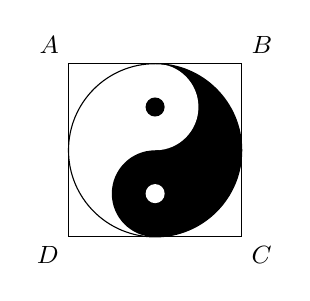
\begin{tikzpicture}[scale=1.1, font=\small]
  % 正方形 ABCD（A 左上、B 右上、C 右下、D 左下），边长 2，内切圆半径 1
  \draw (-1,-1) rectangle (1,1);
  \node[above left]  at (-1, 1) {$A$};
  \node[above right] at ( 1, 1) {$B$};
  \node[below right] at ( 1,-1) {$C$};
  \node[below left]  at (-1,-1) {$D$};
  \begin{scope}
    \clip (0,0) circle (1);
    % 右半黑
    \fill[black] (0,1) arc (90:-90:1) -- cycle;
    % 上小圆白、下小圆黑，构成 S 形分界
    \fill[white] (0,0.5) circle (0.5);
    \fill[black] (0,-0.5) circle (0.5);
    % 鱼眼
    \fill[black] (0,0.5) circle (0.11);
    \fill[white] (0,-0.5) circle (0.11);
  \end{scope}
  \draw (0,0) circle (1);
\end{tikzpicture}
\end{center}
\nopagebreak[4]
\begin{gkopts}(4)
\task A．$\dfrac14$
\task B．$\dfrac\pi8$
\task C．$\dfrac12$
\task D．$\dfrac\pi4$
\end{gkopts}

\end{question}
\begin{question}
\gkti{5}已知 $F$ 是双曲线 $C:x^{2}-\dfrac{y^{2}}3=1$ 的右焦点，$P$ 是 $C$ 上一点，且 $PF$ 与 $x$ 轴垂直，点 $A$ 的坐标是 $(1,3)$，则 $\triangle APF$ 的面积为\mbox{（　　）}

\begin{gkopts}(4)
\task A．$\dfrac13$
\task B．$\dfrac12$
\task C．$\dfrac23$
\task D．$\dfrac32$
\end{gkopts}

\Needspace{0.4\textheight}
\end{question}
\begin{question}
\gkti{6}如图，在下列四个正方体中，$A$，$B$ 为正方体的两个顶点，$M$，$N$，$Q$ 为所在棱的中点，则在这四个正方体中，直线 $AB$ 与平面 $MNQ$ \textbf{不平行}的是\mbox{（　　）}
\nopagebreak[4]
\begin{center}% 2017 全国Ⅰ卷 文6：选项 (A)(B) 的两个正方体
% 前面正方形 (0,0)-(2,2)，后面偏移 (0.85,0.5)；隐藏棱：后左竖棱、左底棱、后底棱
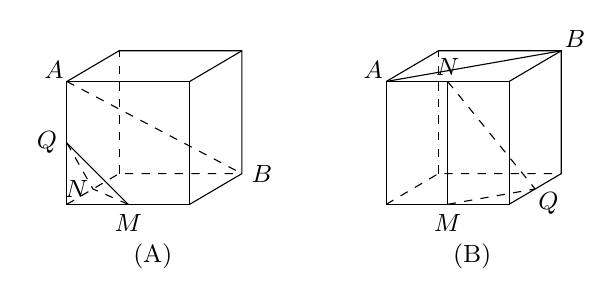
\begin{tikzpicture}[scale=0.78, font=\small]
  % ---------- (A)：A 前左上，B 后右下；M 前下棱中点，N 底面左棱中点，Q 前左竖棱中点 ----------
  \begin{scope}
    \draw (0,0) rectangle (2,2);
    \draw (2,0) -- (2.85,0.5) -- (2.85,2.5) -- (2,2);
    \draw (0,2) -- (0.85,2.5) -- (2.85,2.5);
    \draw[dashed] (0,0) -- (0.85,0.5) -- (2.85,0.5);
    \draw[dashed] (0.85,0.5) -- (0.85,2.5);
    \coordinate (A) at (0,2);
    \coordinate (B) at (2.85,0.5);
    \coordinate (M) at (1,0);
    \coordinate (N) at (0.425,0.25);
    \coordinate (Q) at (0,1);
    \draw[dashed] (A) -- (B);
    \draw (Q) -- (M);
    \draw[dashed] (Q) -- (N) -- (M);
    \node[above left, inner sep=1pt] at (A) {$A$};
    \node[right] at (B) {$B$};
    \node[below] at (M) {$M$};
    \node[left, inner sep=1.5pt] at (N) {$N$};
    \node[left] at (Q) {$Q$};
    \node at (1.4,-0.85) {(A)};
  \end{scope}
  % ---------- (B)：A 前左上，B 后右上；N 前上棱中点，M 前下棱中点，Q 底面右棱中点 ----------
  \begin{scope}[xshift=5.2cm]
    \draw (0,0) rectangle (2,2);
    \draw (2,0) -- (2.85,0.5) -- (2.85,2.5) -- (2,2);
    \draw (0,2) -- (0.85,2.5) -- (2.85,2.5);
    \draw[dashed] (0,0) -- (0.85,0.5) -- (2.85,0.5);
    \draw[dashed] (0.85,0.5) -- (0.85,2.5);
    \coordinate (A) at (0,2);
    \coordinate (B) at (2.85,2.5);
    \coordinate (N) at (1,2);
    \coordinate (M) at (1,0);
    \coordinate (Q) at (2.425,0.25);
    \draw (A) -- (B);
    \draw (N) -- (M);
    \draw[dashed] (N) -- (Q);
    \draw[dashed] (M) -- (Q);
    \node[above left, inner sep=1pt] at (A) {$A$};
    \node[above right, inner sep=1pt] at (B) {$B$};
    \node[above, inner sep=2pt] at (N) {$N$};
    \node[below] at (M) {$M$};
    \node[below right, inner sep=1pt] at (Q) {$Q$};
    \node at (1.4,-0.85) {(B)};
  \end{scope}
\end{tikzpicture}
\end{center}
\nopagebreak[4]
\nopagebreak[4]
\begin{center}% 2017 全国Ⅰ卷 文6：选项 (C)(D) 的两个正方体
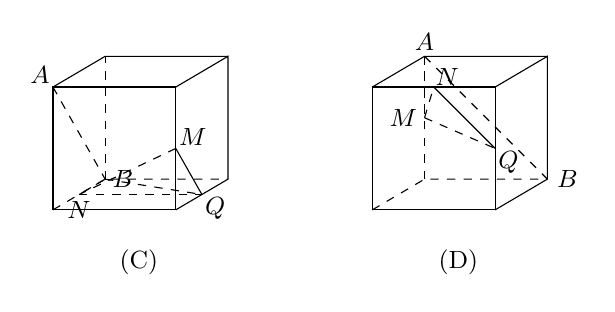
\begin{tikzpicture}[scale=0.78, font=\small]
  % ---------- (C)：A 前左上，B 后左下；M 前右竖棱中点，N 底面左棱中点，Q 底面右棱中点 ----------
  \begin{scope}
    \draw (0,0) rectangle (2,2);
    \draw (2,0) -- (2.85,0.5) -- (2.85,2.5) -- (2,2);
    \draw (0,2) -- (0.85,2.5) -- (2.85,2.5);
    \draw[dashed] (0,0) -- (0.85,0.5) -- (2.85,0.5);
    \draw[dashed] (0.85,0.5) -- (0.85,2.5);
    \coordinate (A) at (0,2);
    \coordinate (B) at (0.85,0.5);
    \coordinate (M) at (2,1);
    \coordinate (N) at (0.425,0.25);
    \coordinate (Q) at (2.425,0.25);
    \draw[dashed] (A) -- (B);
    \draw[dashed] (B) -- (N) (B) -- (Q);   % 到 M N Q 的示意连线在底面/内部
    \draw[dashed] (N) -- (Q);
    \draw (M) -- (Q);
    \draw[dashed] (M) -- (N);
    \node[above left, inner sep=1pt] at (A) {$A$};
    \node[right, inner sep=2.5pt] at (B) {$B$};
    \node[above right, inner sep=1pt] at (M) {$M$};
    \node[below, inner sep=2.5pt] at (N) {$N$};
    \node[below right, inner sep=1pt] at (Q) {$Q$};
    \node at (1.4,-0.85) {(C)};
  \end{scope}
  % ---------- (D)：A 后左上，B 后右下；M 后左竖棱中点，N 前上棱中点，Q 前右竖棱中点 ----------
  \begin{scope}[xshift=5.2cm]
    \draw (0,0) rectangle (2,2);
    \draw (2,0) -- (2.85,0.5) -- (2.85,2.5) -- (2,2);
    \draw (0,2) -- (0.85,2.5) -- (2.85,2.5);
    \draw[dashed] (0,0) -- (0.85,0.5) -- (2.85,0.5);
    \draw[dashed] (0.85,0.5) -- (0.85,2.5);
    \coordinate (A) at (0.85,2.5);
    \coordinate (B) at (2.85,0.5);
    \coordinate (M) at (0.85,1.5);
    \coordinate (N) at (1,2);
    \coordinate (Q) at (2,1);
    \draw[dashed] (A) -- (B);
    \draw[dashed] (A) -- (M);            % A 沿后左竖棱到 M 已被棱覆盖，此线与棱重合
    \draw (N) -- (Q);
    \draw[dashed] (M) -- (N) (M) -- (Q);
    \node[above, inner sep=2pt] at (A) {$A$};
    \node[right] at (B) {$B$};
    \node[left, inner sep=2.5pt] at (M) {$M$};
    \node[above right, inner sep=0.5pt] at (N) {$N$};
    \node[below right, inner sep=1pt] at (Q) {$Q$};
    \node at (1.4,-0.85) {(D)};
  \end{scope}
\end{tikzpicture}
\end{center}
\nopagebreak[4]
\end{question}
\begin{question}
\gkti{7}设 $x$，$y$ 满足约束条件 $\begin{cases}x+3y\le3\\ x-y\ge1\\ y\ge0\end{cases}$，则 $z=x+y$ 的最大值为\mbox{（　　）}

\begin{gkopts}(4)
\task A．$0$
\task B．$1$
\task C．$2$
\task D．$3$
\end{gkopts}

\Needspace{0.4\textheight}
\end{question}
\begin{question}
\gkti{8}函数 $y=\dfrac{\sin2x}{1-\cos x}$ 的部分图象大致为\mbox{（　　）}
\nopagebreak[4]
\begin{center}% 2017 全国Ⅰ卷 文8：y=sin2x/(1-cos x) 图象四选一（正确项 C）
% 全部四个面板均由解析式精确绘制：C=g(x)、A=-g(x)、B=g(|x|)、D=-g(|x|)
% （干扰项表达式为重绘构造，原卷为定性示意图）
\begin{tikzpicture}[font=\footnotesize]
\pgfplotsset{
  panel/.style={width=4.6cm, height=3.8cm, axis lines=middle,
    xmin=-3.6, xmax=3.6, ymin=-3.4, ymax=3.4,
    xtick={-3.14159,1,3.14159}, xticklabels={$-\pi$,$1$,$\pi$},
    ytick={1}, yticklabels={$1$},
    xlabel={$x$}, ylabel={$y$},
    every axis x label/.style={at={(current axis.right of origin)}, anchor=west},
    every axis y label/.style={at={(current axis.above origin)}, anchor=south}}}
  \begin{axis}[panel, at={(0,0)}, name=axA]
    \addplot[domain=0.36:3.14159, samples=150, thick] {-sin(deg(2*x))/(1-cos(deg(x)))};
    \addplot[domain=-3.14159:-0.36, samples=150, thick] {-sin(deg(2*x))/(1-cos(deg(x)))};
    \node[below left] at (axis cs:0,0) {$O$};
  \end{axis}
  \node[below=0.5mm] at (axA.south) {(A)};
  \begin{axis}[panel, at={(5.5cm,0)}, name=axB]
    \addplot[domain=0.36:3.14159, samples=150, thick] {sin(deg(2*abs(x)))/(1-cos(deg(x)))};
    \addplot[domain=-3.14159:-0.36, samples=150, thick] {sin(deg(2*abs(x)))/(1-cos(deg(x)))};
    \node[below left] at (axis cs:0,0) {$O$};
  \end{axis}
  \node[below=0.5mm] at (axB.south) {(B)};
  \begin{axis}[panel, at={(0,-4.9cm)}, name=axC]
    \addplot[domain=0.36:3.14159, samples=150, thick] {sin(deg(2*x))/(1-cos(deg(x)))};
    \addplot[domain=-3.14159:-0.36, samples=150, thick] {sin(deg(2*x))/(1-cos(deg(x)))};
    \node[below left] at (axis cs:0,0) {$O$};
  \end{axis}
  \node[below=0.5mm] at (axC.south) {(C)};
  \begin{axis}[panel, at={(5.5cm,-4.9cm)}, name=axD]
    \addplot[domain=0.36:3.14159, samples=150, thick] {-sin(deg(2*abs(x)))/(1-cos(deg(x)))};
    \addplot[domain=-3.14159:-0.36, samples=150, thick] {-sin(deg(2*abs(x)))/(1-cos(deg(x)))};
    \node[below left] at (axis cs:0,0) {$O$};
  \end{axis}
  \node[below=0.5mm] at (axD.south) {(D)};
\end{tikzpicture}
\end{center}
\nopagebreak[4]
\end{question}
\begin{question}
\gkti{9}已知函数 $f(x)=\ln x+\ln(2-x)$，则\mbox{（　　）}

\begin{gkopts}(2)
\task A．$f(x)$ 在 $(0,2)$ 单调递增
\task B．$f(x)$ 在 $(0,2)$ 单调递减
\task C．$y=f(x)$ 的图象关于直线 $x=1$ 对称
\task D．$y=f(x)$ 的图象关于点 $(1,0)$ 对称
\end{gkopts}

\Needspace{0.4\textheight}
\end{question}
\begin{question}
\gkti{10}如图程序框图是为了求出满足 $3^{n}-2^{n}>1000$ 的最小偶数 $n$，那么在 $\Diamond$ 和 $\square$ 两个空白框中，可以分别填入\mbox{（　　）}
\nopagebreak[4]
\begin{center}% 2017 全国Ⅰ卷 理8/文10：求满足 3^n-2^n>1000 的最小偶数 n 的程序框图
% 两个空白框（菱形与左侧矩形）是题目要求填入的位置，故留白
\begin{tikzpicture}[font=\small, >=Stealth, node distance=8mm,
  box/.style={draw, minimum height=1.9em, inner xsep=7pt},
  term/.style={draw, rounded corners=7pt, minimum height=1.9em, inner xsep=9pt},
  io/.style={draw, trapezium, trapezium left angle=70, trapezium right angle=110,
             minimum height=1.9em, inner xsep=2pt},
  dec/.style={draw, diamond, aspect=2.4, inner sep=1.5pt}]
  \node[term] (start) {开始};
  \node[io, below=of start] (in) {输入 $n=0$};
  \coordinate[below=5mm of in] (merge);
  \node[box, below=2mm of merge] (calc) {$A=3^{n}-2^{n}$};
  \node[dec, below=of calc] (cond) {\phantom{$A\le1000$}};
  \node[box, left=12mm of calc, minimum width=5.2em] (blank) {\phantom{$n=n+2$}};
  \node[io, below=of cond] (out) {输出 $n$};
  \node[term, below=of out] (end) {结束};
  \draw[->] (start) -- (in);
  \draw[->] (in) -- (calc);
  \draw[->] (calc) -- (cond);
  \draw[->] (cond) -- node[right]{否} (out);
  \draw[->] (out) -- (end);
  \draw[->] (cond) -| node[below, pos=0.18]{是} (blank);
  \draw[->] (blank) |- (merge);
\end{tikzpicture}
\end{center}
\nopagebreak[4]
\begin{gkopts}(2)
\task A．$A>1000$ 和 $n=n+1$
\task B．$A>1000$ 和 $n=n+2$
\task C．$A\le1000$ 和 $n=n+1$
\task D．$A\le1000$ 和 $n=n+2$
\end{gkopts}

\begin{gktip}
\textbf{注}：程序框图（算法初步）在现行新课标中已删除。
\end{gktip}

\end{question}
\begin{question}
\gkti{11}$\triangle ABC$ 的内角 $A$，$B$，$C$ 的对边分别为 $a$，$b$，$c$，已知 $\sin B+\sin A(\sin C-\cos C)=0$，$a=2$，$c=\sqrt2$，则 $C=$\mbox{（　　）}

\begin{gkopts}(4)
\task A．$\dfrac\pi{12}$
\task B．$\dfrac\pi6$
\task C．$\dfrac\pi4$
\task D．$\dfrac\pi3$
\end{gkopts}

\end{question}
\begin{question}
\gkti{12}设 $A$，$B$ 是椭圆 $C:\dfrac{x^{2}}3+\dfrac{y^{2}}m=1$ 长轴的两个端点。若 $C$ 上存在点 $M$ 满足 $\angle AMB=120^\circ$，则 $m$ 的取值范围是\mbox{（　　）}

\begin{gkopts}(2)
\task A．$(0,1]\cup[9,+\infty)$
\task B．$\left(0,\sqrt3\right]\cup[9,+\infty)$
\task C．$(0,1]\cup[4,+\infty)$
\task D．$\left(0,\sqrt3\right]\cup[4,+\infty)$
\end{gkopts}

\par\medskip

\end{question}
\gkpart{二、填空题}

\begin{gktip}
本题共 4 小题，每小题 5 分，共 20 分。
\end{gktip}

\begin{question}
\gkti{13}已知向量 $\boldsymbol a=(-1,2)$，$\boldsymbol b=(m,1)$。若向量 $\boldsymbol a+\boldsymbol b$ 与 $\boldsymbol a$ 垂直，则 $m=$ \gkblank{}．

\end{question}
\begin{question}
\gkti{14}曲线 $y=x^{2}+\dfrac1x$ 在点 $(1,2)$ 处的切线方程为 \gkblank{}．

\end{question}
\begin{question}
\gkti{15}已知 $\alpha\in\left(0,\dfrac\pi2\right)$，$\tan\alpha=2$，则 $\cos\left(\alpha-\dfrac\pi4\right)=$ \gkblank{}．

\end{question}
\begin{question}
\gkti{16}已知三棱锥 $S\text{-}ABC$ 的所有顶点都在球 $O$ 的球面上，$SC$ 是球 $O$ 的直径。若平面 $SCA\perp$ 平面 $SCB$，$SA=AC$，$SB=BC$，三棱锥 $S\text{-}ABC$ 的体积为 $9$，则球 $O$ 的表面积为 \gkblank{}．

\par\medskip

\end{question}
\gkpart{三、解答题}

\begin{gktip}
共 70 分。第 17～21 题为必考题，第 22、23 题为选考题。
\end{gktip}

\gksubpart{（一）必考题：共 60 分}

\begin{question}
\gkti{17}\textbf{（12 分）} 记 $S_n$ 为等比数列 $\left\{a_n\right\}$ 的前 $n$ 项和。已知 $S_2=2$，$S_3=-6$。

  (1) 求 $\left\{a_n\right\}$ 的通项公式；

  (2) 求 $S_n$，并判断 $S_{n+1}$，$S_n$，$S_{n+2}$ 是否能成等差数列。

\Needspace{0.4\textheight}
\end{question}
\begin{question}
\gkti{18}\textbf{（12 分）} 如图，在四棱锥 $P\text{-}ABCD$ 中，$AB\parallel CD$，且 $\angle BAP=\angle CDP=90^\circ$。
\nopagebreak[4]
\begin{center}% 2017 全国Ⅰ卷 理18/文18：四棱锥 P-ABCD（AB∥CD，∠BAP=∠CDP=90°）
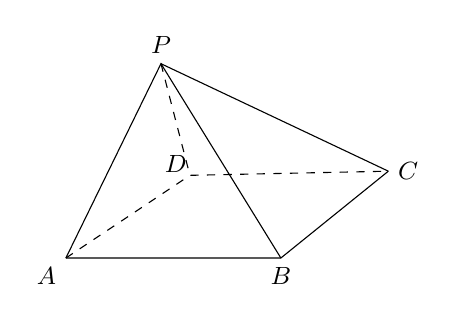
\begin{tikzpicture}[scale=1.05, font=\small]
  \coordinate (P) at (1.15,2.35);
  \coordinate (A) at (0,0);
  \coordinate (B) at (2.6,0);
  \coordinate (C) at (3.9,1.05);
  \coordinate (D) at (1.5,1.0);
  \draw (A) -- (B) -- (C);
  \draw (A) -- (P) -- (B);
  \draw (P) -- (C);
  \draw[dashed] (A) -- (D) -- (C);
  \draw[dashed] (P) -- (D);
  \node[above] at (P) {$P$};
  \node[below left] at (A) {$A$};
  \node[below] at (B) {$B$};
  \node[right] at (C) {$C$};
  \node[above left, inner sep=1pt] at (D) {$D$};
\end{tikzpicture}
\end{center}
\nopagebreak[4]
  (1) 证明：平面 $PAB\perp$ 平面 $PAD$；

  (2) 若 $PA=PD=AB=DC$，$\angle APD=90^\circ$，且四棱锥 $P\text{-}ABCD$ 的体积为 $\dfrac83$，求该四棱锥的侧面积。

\end{question}
\begin{question}
\gkti{19}\textbf{（12 分）} 为了监控某种零件的一条生产线的生产过程，检验员每隔 $30\ \min$ 从该生产线上随机抽取一个零件，并测量其尺寸（单位：$\mathrm{cm}$）。下面是检验员在一天内依次抽取的 $16$ 个零件的尺寸：

\begin{center}
\begingroup\setlength{\tabcolsep}{4pt}
\begin{tabular}{ccccccccc}
\toprule
抽取次序 & $1$ & $2$ & $3$ & $4$ & $5$ & $6$ & $7$ & $8$ \\
\midrule
零件尺寸 & $9.95$ & $10.12$ & $9.96$ & $9.96$ & $10.01$ & $9.92$ & $9.98$ & $10.04$ \\
\bottomrule
\end{tabular}
\endgroup
\end{center}

\begin{center}
\begingroup\setlength{\tabcolsep}{4pt}
\begin{tabular}{ccccccccc}
\toprule
抽取次序 & $9$ & $10$ & $11$ & $12$ & $13$ & $14$ & $15$ & $16$ \\
\midrule
零件尺寸 & $10.26$ & $9.91$ & $10.13$ & $10.02$ & $9.22$ & $10.04$ & $10.05$ & $9.95$ \\
\bottomrule
\end{tabular}
\endgroup
\end{center}

经计算得

\nopagebreak[4]
\[\bar x=\frac1{16}\sum_{i=1}^{16}x_i=9.97,\qquad s=\sqrt{\frac1{16}\sum_{i=1}^{16}\left(x_i-\bar x\right)^{2}}=\sqrt{\frac1{16}\left(\sum_{i=1}^{16}x_i^{2}-16\bar x^{2}\right)}\approx0.212\]

\nopagebreak[4]
\[\sqrt{\sum_{i=1}^{16}(i-8.5)^{2}}\approx18.439,\qquad \sum_{i=1}^{16}\left(x_i-\bar x\right)(i-8.5)=-2.78\]

其中 $x_i$ 为抽取的第 $i$ 个零件的尺寸，$i=1,2,\cdots,16$。

  (1) 求 $\left(x_i,\ i\right)\ (i=1,2,\cdots,16)$ 的相关系数 $r$，并回答是否可以认为这一天生产的零件尺寸不随生产过程的进行而系统地变大或变小（若 $|r|<0.25$，则可以认为零件的尺寸不随生产过程的进行而系统地变大或变小）；

  (2) 一天内抽检零件中，如果出现了尺寸在 $(\bar x-3s,\ \bar x+3s)$ 之外的零件，就认为这条生产线在这一天的生产过程可能出现了异常情况，需对当天的生产过程进行检查。

  　① 从这一天抽检的结果看，是否需对当天的生产过程进行检查？

  　② 在 $(\bar x-3s,\ \bar x+3s)$ 之外的数据称为离群值，试剔除离群值，估计这条生产线当天生产的零件尺寸的均值与标准差（精确到 $0.01$）。

  附：样本 $\left(x_i,y_i\right)\ (i=1,2,\cdots,n)$ 的相关系数

\nopagebreak[4]
\[r=\frac{\sum\limits_{i=1}^{n}\left(x_i-\bar x\right)\left(y_i-\bar y\right)}{\sqrt{\sum\limits_{i=1}^{n}\left(x_i-\bar x\right)^{2}}\sqrt{\sum\limits_{i=1}^{n}\left(y_i-\bar y\right)^{2}}},\qquad \sqrt{0.008}\approx0.09\]

\end{question}
\begin{question}
\gkti{20}\textbf{（12 分）} 设 $A$，$B$ 为曲线 $C:y=\dfrac{x^{2}}4$ 上两点，$A$ 与 $B$ 的横坐标之和为 $4$。

  (1) 求直线 $AB$ 的斜率；

  (2) 设 $M$ 为曲线 $C$ 上一点，$C$ 在 $M$ 处的切线与直线 $AB$ 平行，且 $AM\perp BM$，求直线 $AB$ 的方程。

\end{question}
\begin{question}
\gkti{21}\textbf{（12 分）} 已知函数 $f(x)=\mathrm e^{x}\left(\mathrm e^{x}-a\right)-a^{2}x$。

  (1) 讨论 $f(x)$ 的单调性；

  (2) 若 $f(x)\ge0$，求 $a$ 的取值范围。

\par\medskip

\end{question}
\gksubpart{（二）选考题：共 10 分，第 22、23 题任选一题作答}

\begin{gktip}
\textbf{ 现行考纲已取消选做题}，以下两题仅作历史资料保留。
\end{gktip}

\begin{question}
\gkti{22}\textbf{（10 分）〔选修 4-4：坐标系与参数方程〕} （\textbf{已取消}）

在直角坐标系 $xOy$ 中，曲线 $C$ 的参数方程为 $\begin{cases}x=3\cos\theta\\ y=\sin\theta\end{cases}$（$\theta$ 为参数），直线 $l$ 的参数方程为 $\begin{cases}x=a+4t\\ y=1-t\end{cases}$（$t$ 为参数）。

  (1) 若 $a=-1$，求 $C$ 与 $l$ 的交点坐标；

  (2) 若 $C$ 上的点到 $l$ 距离的最大值为 $\sqrt{17}$，求 $a$。

\end{question}
\begin{question}
\gkti{23}\textbf{（10 分）〔选修 4-5：不等式选讲〕} （\textbf{已取消}）

已知函数 $f(x)=-x^{2}+ax+4$，$g(x)=|x+1|+|x-1|$。

  (1) 当 $a=1$ 时，求不等式 $f(x)\ge g(x)$ 的解集；

  (2) 若不等式 $f(x)\ge g(x)$ 的解集包含 $[-1,1]$，求 $a$ 的取值范围。

\par\medskip


\end{question}